%-------------------------------------------------------------------------------
\chapter[Non-cohesive and cohesive suspended sediment transport]{Non-cohesive and cohesive suspended sediment transport}\label{sec:SuspendedSedimentTransport}
%-------------------------------------------------------------------------------

%-------------------------------------------------------------------------------
\section{Preliminaries}
%-------------------------------------------------------------------------------
The suspended load is the portion of the sediment that is carried by a fluid flow which settle slowly enough such that it almost never touches the bed. It is maintained in suspension by the turbulence in the flowing water and consists of particles generally of the fine sand, silt and clay size. An exhaustive analysis of this topic can be found in~\cite{GarciaBook2006} and references therein.

%-------------------------------------------------------------------------------
\section{Non-cohesive sediment transport}
%-------------------------------------------------------------------------------

Suspended sediment transport is accounted by \gaia{} by solving the two-dimensional advection-diffusion equation, expressed by:
\begin{equation}\label{eq:2DADE}
\frac{\partial hC}{\partial t} + \frac{\partial hUC}{\partial x} + \frac{\partial hVC}{\partial y} =
\frac{\partial}{\partial x}\left(h\epsilon_s\frac{\partial C}{\partial x}\right) +
\frac{\partial}{\partial y}\left(h\epsilon_s\frac{\partial C}{\partial y}\right) + E-D
\end{equation}
where $C=C(x,y,t)$ is the depth-averaged concentration \textcolor{black}{\bf expressed in \% volume (-)}, $(U,V)$ are the depth-averaged components of the velocity in the $x$ and $y$ directions, respectively, $\epsilon_s$ is the turbulent diffusivity of the sediment, often related to the eddy viscosity $\epsilon_s=\nu_t/\sigma_c$, with $\sigma_c$ the Schmidt number. In \gaia{}, $\sigma_c=1.0$.

The non-cohesive deposition rate is $D = w_s C_{z_{ref}}$, where $w_s$ is the settling velocity and $C_{z_{ref}}$ is the near-bed concentration, evaluated at the interface between the bed load
and the suspended load, $z=z_{ref}$.\\

The non-cohesive erosion rate is $E = w_s C_{eq}$, where $C_{eq}$ is the equilibrium near-bed concentration determined by using an empirical formula.

For non-cohesive sediments, the net sediment flux $E-D$ is therefore determined based on the concept of equilibrium concentration, see~\cite{CelikRodi}:
\begin{equation}\label{eq:CelikRodi}
\left(E-D \right)_{z_{ref}} = w_s \left(C_{eq} - C_{z_{ref}}\right).
\end{equation}

In \gaia{} it is assumed a Rouse profile for the vertical concentration distribution,
which is theoretically valid in uniform steady flow conditions:
\begin{equation}\label{eq:Rouseprofile}
C(z)=C_{z_{ref}}\left(\frac{z-h}{z}\frac{a}{a-h}\right)^R,
\end{equation}
where $R$ is the Rouse number defined by
\begin{equation}\label{eq:R}
R=\frac{w_s}{\kappa u_*},
\end{equation}
with $\kappa$ the von Karman constant ($\kappa = 0.4$), $u_*$ the
friction velocity corresponding to the total bed shear stress, and $a$ the reference elevation above the bed elevation. The distance $a$, defined variously by
various authors, is taken to be very close to the bed.

By depth-integration of the Rouse profile (\ref{eq:Rouseprofile}), the following relation
can be established between the depth-averaged concentration and the reference concentration:
\begin{equation*}
  C_{z_{ref}} = F C,
\end{equation*}
where:
\begin{equation}\label{eq:Rouseprofile}
F^{-1} = \left(\frac{z_{ref}}{h}\right)^R\int_{z_{ref}/h}^1\left(\frac{1-u}{u}\right)^R du.
\end{equation}
In \gaia{}, the following expression is used to compute $F$:

\begin{equation*}
F^{-1}=\left\{\begin{array}{ll}
\frac{1}{\left(1-Z\right)} B^R\left( 1-B^{(1-R)} \right) & \text{if}\,R \neq 1\\
-B \log B &  \text{if}\,R = 1
\end{array}
\right.
\end{equation*}
with $B = z_{ref}/h$.

By considering suspended sediment transport, the bed evolution is computed by: %... CHECK!!!!!$\rho_s$???
\begin{equation*}
(1-\lambda)\frac{\partial z_b}{\partial t} = D - E
\end{equation*}
with $\lambda$ the bed porosity, and $z_b$ the bed level.



%...............................................................................
\subsection{Available equilibrium near-bed concentration formulas}\label{sec:concform}
%...............................................................................
\subsubsection{Zyserman-Fredsoe}
\begin{itemize}
\item The Zyserman-Fredsoe formula~\cite{Zyserman} \telkey{REFERENCE CONCENTRATION FORMULA = 1}
\begin{equation*}
C_{eq} =\frac{0.331(\theta'-\theta_{cr})^{1.75}}{1+0.72(\theta'-\theta_{cr})^{1.75}},
\end{equation*}
where $\theta_{cr}$ is the critical Shields parameter and $\theta'= \mu\theta$ the shear stress due to skin friction (see \S\ref{sec:skin}).
\item The reference elevation $z_{ref}=\alpha_{k_s}\times d_{50}$ ($=3.0\times d_{50}$ by default, $\alpha_{k_s}$ can be modified with the keyword \telkey{ RATIO BETWEEN SKIN FRICTION AND MEAN DIAMETER})
\item Fortran subroutine {\ttfamily suspension\_fredsoe.f}.
\end{itemize}

\subsubsection{Bijker}
\begin{itemize}
\item Bijker formula \telkey{REFERENCE CONCENTRATION FORMULA = 2}
\item This formula is related to the bedload sediment transport $Q_b$, therefore this option cannot be used without activating the bedload transport mechanism \telkey{ BED LOAD = YES}, with \telkey{ COUPLING PERIOD FOR gaia = 1}
\begin{equation*}
C_{eq} =\frac{Q_b}{b\,z_{ref}\,u_*}
\end{equation*}
with $b$ a constant ($=6.34$) and $u_*$ the shear velocity
\item The reference elevation $z_{ref}=k_{sr}$, with $k_{sr}$ the rippled bed roughness
\item Fortran subroutine {\ttfamily suspension\_bijker.f}.
\end{itemize}

\subsubsection{van Rijn}
\begin{itemize}
\item van Rijn formula~\cite{vanRijn84b} \telkey{REFERENCE CONCENTRATION FORMULA = 3}
\begin{equation*}
C_{eq} =0.015\,d_{50}\frac{\left(\theta'/\theta_{cr}-1\right)^{3/2}}{z_{ref}D_*^{0.3}}
\end{equation*}
with $\theta_{cr}$ the critical Shields parameter and and $\theta'= \mu\theta$ the shear stress due to skin friction.
\item The reference elevation $z_{ref}=0.5 \times k_s$, with $k_s$ the total roughness (from the hydrodynamics steering file)
\item Fortran subroutine {\ttfamily suspension\_vanrijn.f}.
\end{itemize}

\subsubsection{Soulsby \& van Rijn}
\begin{itemize}
\item Soulsby and van Rijn formula~\cite{Soulsby97} \telkey{REFERENCE CONCENTRATION FORMULA = 4}
  \begin{equation*}
C_{eq}=\left\{\begin{array}{ll}
A_{ss}\left(\sqrt{U_c^2+\frac{0.018}{C_D}U_w^2-U_{cr}}\right)^{2.4} & \text{if}\, \geq U_{cr}\\
0.0 &  \text{otherwise}
\end{array}
\right.
\end{equation*}
  with $U_c$ the norm of the depth-averaged current velocity and $U_w$ the wave orbital velocity (see Chapter~\ref{ch:sed_waves}). The threshold current velocity $U_{cr}$ is computed as:
\begin{equation*}
U_{cr}=\left\{\begin{array}{ll}
  0.19 (d_{50}^{0.1})\log_{10}\left(\frac{4.0 h}{d_{90}}\right) & \text{if}\, d_{50} < 0.0005 m\\
  8.5 (d_{50}^{0.6})\log_{10}\left(\frac{4.0 h}{d_{90}}\right) & \text{otherwise}\\
\end{array}
\right.
\end{equation*}
with $d_{90}$ the particle diameter representing the 90\% cummulative percentile value (90\% of the particles in the sediment sample are finer than the $d_{90}$ grain size), in meters.

If wave effects are considered, the quadratic drag coefficient $C_D$ is computed as follows:
\begin{equation*}
  C_D = \left(\frac{0.4}{\log(\max(h, z_{0})/z_{0}-1)}\right)^{2},
\end{equation*}
with $z_{0}=0.006$m the bed roughness.

The empirical suspended transport factor $A_{ss}$ is computed by:
\begin{equation*}
A_{ss} = \frac{0.012 h d_{50} \left(\left(\frac{g(s-1)}{\nu^2}\right)^{1/3}d_{50}\right)^{-0.6}}{\left((s-1)g d_{50}\right)^{1.2}}
\end{equation*}
\item Fortran subroutine {\ttfamily suspension\_sandflow.f}.
\end{itemize}

%-------------------------------------------------------------------------------
\section{Cohesive sediment transport}
%-------------------------------------------------------------------------------
Cohesive properties appear for fine particles (silts and clay), with diameter less than a limiting value of about 60 $\mu$m, depending on the physico-chemical
properties of the fluid and salinity. The separation value at $60\mu$m to discriminate non-cohesive from cohesive sediment is conventional. This value is different depending on the country (e.g. $63\mu$m in The Netherlands, $75\mu$m in USA as pointed by Winterwerp and Van Kesteren~\cite{Winterwerp}). Moreover, aggregation of flocs can lead to the formation of macro-flocs larger than $100\mu$m.\\

Fine cohesive sediments are mainly transported in suspension and transport processes strongly depend on the state of floculation of the suspension and consolidation of the bed. The erosion rate mainly depends on the degree of consolidation of the sediment bed, while the settling velocity depends on the state of floculation and aggregates properties.\\

In \gaia{}, cohesive sediments are accounted by solving the 2D advection-diffusion equation:
\begin{equation*}
\frac{\partial hC}{\partial t} + \frac{\partial hUC}{\partial x} + \frac{\partial hVC}{\partial y} =
\frac{\partial}{\partial x}\left(h\epsilon_s\frac{\partial C}{\partial x}\right) +
\frac{\partial}{\partial y}\left(h\epsilon_s\frac{\partial C}{\partial y}\right) + (E-D)
\end{equation*}
$C=C(x,y,t)$ is the depth-averaged concentration \textcolor{black}{expressed in \% volume (-)}, $(U,V)$ are the depth-averaged components of the velocity in the $x$ and $y$ directions, respectively, $\epsilon_s$ is the turbulent diffusivity of the sediment.

The erosion flux is computed with the Partheniades formula:
\begin{equation*}
E = \left\{\begin{array}{ll}
M\left[\left(\frac{\tau_b}{\tau_{ce}}\right)-1\right]\quad & \text{if}\,\,\tau_b> \tau_{ce}\\
0\quad & \text{otherwise}
\end{array}
\right.
\end{equation*}
with $M$ the Krone-Partheniades erosion law constant [kg/m$^2$/s] and $\tau_{ce}$ the critical bed shear stress.

The deposition flux for mud is computed by the expression:
\begin{equation}
D = w_{s} C \left[1-\left(\frac{\sqrt{\tau_b/\rho}}{u_{*mud}^{cr}}\right)^2 \right],
\end{equation}
where $u_{*mud}^{cr}$ is the critical shear velocity for mud deposition.\\

The bed evolution is computed by:
\begin{equation*}
(1-\lambda)\frac{\partial z_b}{\partial t} = D - E
\end{equation*}
with $\lambda$ the bed porosity and $z_b$ bed level.

%-------------------------------------------------------------------------------
\subsection{Initialization of the bed structure}
%-------------------------------------------------------------------------------
The cohesive sediment bed can be represented by a fixed number of layers ($<20$) with the keyword {\ttfamily NUMBER OF LAYERS OF THE CONSOLIDATION MODEL} (integer type, set to {\ttfamily = 1} by default).

Each layer is characterized by its concentration and resistance to the erosion. The concentration of each layer $C_s$ is generally constant and can be specified with the keyword {\ttfamily MUD CONCENTRATION PER LAYER} (real list, set to {\ttfamily = 50.;100.;150.;...} by default), expressed in kg/m$^3$ or gr/l.

The resistance of each layer can be specified with the keyword {\ttfamily CRITICAL EROSION SHEAR STRESS OF THE MUD} (real list, set to {\ttfamily = 0.01;0.02;0.03;...} by default), expressed in N/m$^2$.

The initialization can also be done with the subroutine \texttt{init\_compo\_coh.f}.

\begin{figure}[H]%
\begin{center}
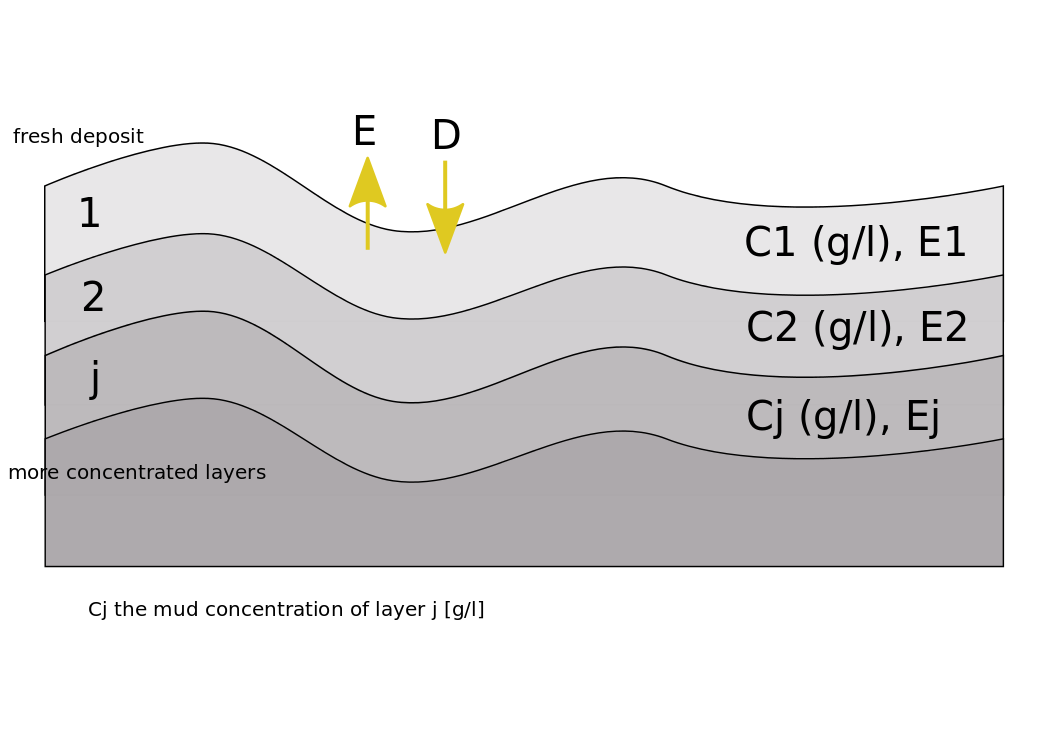
\includegraphics[scale=0.3]{./graphics/consolidation.png}
\end{center}
\end{figure}

%-------------------------------------------------------------------------------
\subsection{Properties of the cohesive sediments}
%-------------------------------------------------------------------------------
The keywords {\ttfamily NUMBER OF BED LOAD MODEL LAYERS} (for non-cohesive sediments) and {\ttfamily NUMBER OF LAYERS OF THE CONSOLIDATION MODEL} are essentially the same except that the default values are different. For cohesive sediments, it is possible to have only one uniform layer, whereas for non-cohesive sand grading we need at least two layers (the active layer and the stratum).
For uniform beds the following keywords need to be specified: {\ttfamily NUMBER OF BED LOAD MODEL LAYERS = 1}\\
and {\ttfamily NUMBER OF LAYERS OF THE CONSOLIDATION MODEL = 1}.

%-------------------------------------------------------------------------------
\subsubsection{Erosion flux}
%-------------------------------------------------------------------------------
The erosion flux is computed with the Partheniades formula. For uniform beds, the erosion flux is related to the excess of
applied bed shear stress to the bed shear strength at the bed surface:
\begin{equation*}
E = \left\{\begin{array}{ll}
M\left[\left(\frac{\tau_b}{\tau_{ce}}\right)-1\right]\quad & \text{if}\,\,\tau_b> \tau_{ce}\\
0\quad & \text{otherwise}
\end{array}
\right.
\end{equation*}
where $M$ the Krone-Partheniades erosion law constant [kg/m$^2$/s] is provided by the keyword {\ttfamily PARTHENIADES CONSTANT} (real type, set to {\ttfamily = 1.E-03} by default).

The value of $\tau_{ce}$ can be provided for the different layers with the keyword {\ttfamily CRITICAL EROSION SHEAR STRESS OF THE MUD} (real list, set to {\ttfamily = 0.01;0.02;0.03;...} by default), expressed in N/m$^2$.

%-------------------------------------------------------------------------------
\subsubsection{Deposition flux}
%-------------------------------------------------------------------------------
The deposition flux for mud is computed by the expression:
\begin{equation}
D = w_{s} C \left[1-\left(\frac{\sqrt{\tau_b/\rho}}{u_{*mud}^{cr}}\right)^2 \right],
\end{equation}
where $u_{*mud}^{cr}$ is the critical shear velocity for mud deposition, expressed in [m/s] and provided by the keyword {\ttfamily CRITICAL SHEAR VELOCITY FOR MUD DEPOSITION} (real type, set to {\ttfamily = 1000.} by default).

For the evaluation of the settling velocity $w_s $, if the keyword {\ttfamily SETTLING VELOCITIES} is not included in the steering file, \gaia{} computes the settling velocity for each sediment class by the Stokes, Zanke or van Rijn formulae depending on the grain size. For further details see the subroutine \texttt{vitchu\_gaia.f}.


%-------------------------------------------------------------------------------
\section{Non-uniform suspended sediment transport}
%-------------------------------------------------------------------------------

%...............................................................................
\section{Initial and boundary conditions for suspended sediment transport}
%...............................................................................
The initial condition value of the concentration can be specified through the keyword \telkey{INITIAL SUSPENSION CONCENTRATIONS} (real type list, {\ttfamily = 0.0} by default). This keyword is not considered if \texttt{EQUILIBRIUM INFLOW CONCENTRATION = YES}.\\

The specification of boundary conditions is done in a boundary condition file, usually named with extension \texttt{*.cli}. The reader is referred to \S\ref{sec:flags} for the definition of the different flags used in the boundary condition file.

\subsection{Wall boundary conditions}
At banks and islands, the suspended load concentration gradients are set to zero. For this case, the flag \texttt{LIEBOR} is set \texttt{= 2} as shown in the example below:

\begin{lstlisting}[frame=trBL]
2 2 2 0.0 0.0 0.0 0.0 (*@\color{PantoneRed}2@*) 0.0 0.0 0.0 565 1
\end{lstlisting}

\subsection{Inflow boundary conditions}
Different ways to impose the concentration at inflow boundary conditions are proposed in \gaia. For this case, the flag \texttt{LICBOR} is set \texttt{= 5}, with the following options for the concentration values:
\begin{itemize}
\item Specified in the column \texttt{CBOR}. In the example below, a \textcolor{black}{\textbf{depth-averaged volume concentration value}} {\ttfamily = 1.0} is provided:
\begin{lstlisting}[frame=trBL]
4 5 5 0.0 0.0 0.0 0.0 (*@\color{PantoneRed}5@*) (*@\color{PantoneRed}1.0@*) 0.0 0.0 565 1
\end{lstlisting}
\item Specified by the \textcolor{black}{\textbf{depth-averaged volume concentration values}} at the boundary through the keyword \telkey{CONCENTRATION PER CLASS AT BOUNDARIES} (real type list of size equal to the number of boundaries $\times$ the number of sediment classes):
\begin{lstlisting}[frame=trBL]
4 5 5 0.0 0.0 0.0 0.0 (*@\color{PantoneRed}5@*) 0.0 0.0 0.0 565 1
\end{lstlisting}
\begin{lstlisting}[frame=trBL]
CONCENTRATION PER CLASS AT BOUNDARIES = 0.0; 0.0; 1.0; ...
\end{lstlisting}
The order is the following: boundary 1 (class 1, class2, etc.), then boundary 2, etc.
\item Computed by \gaia{} through the keyword \telkey{EQUILIBRIUM INFLOW CONCENTRATION} (logical type variable, {\ttfamily = NO} by default) and according to the choice of the formula of equilibrium near-bed concentration (\telkey{REFERENCE CONCENTRATION FORMULA = 1} by default)
\begin{lstlisting}[frame=trBL]
4 5 5 0.0 0.0 0.0 0.0 (*@\color{PantoneRed}5@*) 0.0 0.0 0.0 565 1
\end{lstlisting}
\begin{lstlisting}[frame=trBL]
EQUILIBRIUM INFLOW CONCENTRATION = YES
REFERENCE CONCENTRATION FORMULA = 1
\end{lstlisting}
\item Time-varying {\textbf{depth-averaged mass concentration values}} provided in an external ascii file through the keyword \telkey{LIQUID BOUNDARIES FILE}:
\begin{lstlisting}[frame=trBL]
4 5 5 0.0 0.0 0.0 0.0 (*@\color{PantoneRed}5@*) 0.0 0.0 0.0 565 1
\end{lstlisting}
\begin{lstlisting}[frame=trBL]
LIQUID BOUNDARIES FILE = '<file name>'
\end{lstlisting}
\end{itemize}

According to the hydrodynamic forcing, the use of the keyword \telkey{EQUILIBRIUM INFLOW CONCENTRATION} can be used to prevent the excessive erosion and deposition on the inflow boundary.

\subsection{Outflow boundary conditions}
At the outflow boundary, the suspended load concentration gradient in the flow direction is set to zero. For this case, the flag \texttt{LICBOR} is set \texttt{= 4} as shown in the example below:

\begin{lstlisting}[frame=trBL]
5 4 4 0.0 0.0 0.0 0.0 (*@\color{PantoneRed}4@*) 0.0 0.0 0.0 565 1
\end{lstlisting}

Stability issues at inflow boundaries can be solved by activating the keyword \telkey{TREATMENT OF FLUXES AT THE BOUNDARIES} (integer type variable, {\ttfamily = 2}, default option). The choice {\ttfamily = 1} can be activated when prescribed values are provided. The choice {\ttfamily = 2} is used when fluxes are imposed.

%...............................................................................
\section{Mass and volume concentration}
%...............................................................................
\begin{itemize}
\item Values given through the keyword \telkey{ CONCENTRATION PER CLASS AT BOUNDARIES} must be expressed by \textcolor{black}{\textbf{volume concentration}} $[-]$
\item Values given through the external file must be expressed by {\textbf{mass concentration}} $[$g$/$l$]$ or $[$kg$/$m$^3]$
\item The keyword \telkey{ MASS CONCENTRATION} (logical type variable, {\ttfamily = NO} by default) is only used for printout purposes (results file).
\end{itemize}

%...............................................................................
\section{Diffusion and dispersion}
%...............................................................................
The diffusion term in the ADE for the depth-averaged suspended concentration is taken into account with the keyword \telkey{ DIFFUSION} (logical type, set {\ttfamily = YES} by default). The values of the diffusion coefficients can be specified with the keyword \telkey{ OPTION FOR THE DISPERSION} (integer type, set {\ttfamily = 1} by default), with the following options:
\begin{itemize}
\item {\ttfamily = 1}: values of the longitudinal and transversal dispersion coefficients are provided with the keywords \texttt{DISPERSION ALONG THE FLOW} and \texttt{DISPERSION ACROSS THE FLOW}, respectively:
\begin{itemize}
\item \telkey{DISPERSION ALONG THE FLOW} (real type, set {\ttfamily = $1.0 \times 10^{-2}$ m$^2/$s} by default)
\item \telkey{DISPERSION ACROSS THE FLOW} (real type, set {\ttfamily = $1.0 \times 10^{-2}$ m$^2/$s} by default)
\end{itemize}

\item {\ttfamily = 2}: values of the longitudinal and transversal dispersion coefficients are computed with the Elder model $T_l=\alpha_l u_* h$ and $T_t=\alpha_t u_* h$, where the coefficients $\alpha_l$ and $\alpha_t$ can be provided with the keywords \texttt{DISPERSION ALONG THE FLOW} and \texttt{DISPERSION ACROSS THE FLOW}.
\item {\ttfamily = 3}: values of the dispersion coefficients are provided by the hydrodynamics module (e.g. \telemac{2D})
\end{itemize}

%...............................................................................
\section{Numerical treatment of the diffusion terms}
%...............................................................................
The keyword \texttt{OPTION FOR THE DIFFUSION OF TRACER} (integer type, set {\ttfamily = 1} by default) allows to choose the treatment of the diffusion terms in the advection-diffusion equation \ref{eq:2DADE} for the depth-averaged suspended concentration:
\begin{itemize}
\item \texttt{= 1}: the diffusion term is solved in the form $\nabla\cdot(\varepsilon_s\nabla T)$
\item \texttt{= 2}: the diffusion term is solved in the form $\frac{1}{h}\nabla\cdot(h\varepsilon_s\nabla T)$
\end{itemize}

%...............................................................................
\section{Numerical treatment of the advection terms}
%...............................................................................
The choice for the scheme for the treatment of the advection terms can be done with the keyword \texttt{TYPE OF ADVECTION} (integer type, set {\ttfamily = 1} by default):
\begin{lstlisting}[frame=trBL]
1="CHARACTERISTICS"
2="SUPG"
3="CONSERVATIVE N-SCHEME"
4="CONSERVATIVE N-SCHEME"
5="CONSERVATIVE PSI-SCHEME"
6="NON CONSERVATIVE PSI SCHEME"
7="IMPLICIT NON CONSERVATIVE N SCHEME"
13="EDGE-BASED N-SCHEME"
14="EDGE-BASED N-SCHEME"
15="ERIA SCHEME"
\end{lstlisting}

\begin{WarningBlock}{Note:}
  It is recommended to use the schemes {\ttfamily 4} or {\ttfamily 14} for a good compromise between accuracy and computational time (specially if tidal flats are present). It is also suggested to active
  the keyword \texttt{CONTINUITY CORRECTION = YES}.
\end{WarningBlock}

A brief description of the numerical schemes implemented in \gaia{} is given below:
\begin{itemize}
\item \textbf{Method of characteristics} (\texttt{1})
\begin{itemize}
\item Unconditionally stable and monotonous
\item Diffusive for small time steps, Not conservative
\end{itemize}
\item \textbf{Method Streamline Upwind Petrov Galerkin SUPG} (\texttt{2})
\begin{itemize}
\item Based on the Courant number criteria
\item Less diffusive for small time steps, Not conservative
\end{itemize}
\item \textbf{Conservative N-scheme (similar to finite volumes)} (\texttt{3, 4})
\begin{itemize}
\item Solves the continuity equation under its conservative form
\item Recommended for correction on convection velocity
\item Courant number limitation (sub-iterations to reduce time step)
\end{itemize}
\item \textbf{Edge-based N-scheme} (\texttt{13, 14})
\begin{itemize}
\item Same as \texttt{3} and \texttt{4} but adapted to tidal flats
\item Based on positive-depth algorithm
\end{itemize}
\item \textbf{Distributive schemes PSI} (\texttt{5, 6})
\begin{itemize}
\item fluxes corrected according to the tracer value: relaxation of Courant number criteria, less diffusive than
schemes \texttt{4, 14} but larger CPU time
\item Should not be applied for tidal flats
\end{itemize}
\item \textbf{Eria scheme} (\texttt{15})
\begin{itemize}
\item Works for tidal flats
\end{itemize}
\end{itemize}
For further information about these schemes, refer to \telemac{2d} user's manual.

\subsection{Correction of the convection velocity}
As most of the sediment transport processes occur near the bed, it often exhibits an over-estimation of suspended sand transport.
A correction method accounting for the vertical velocity and concentration profiles is therefore proposed. A straightforward treatment of the advection terms would imply the
definition of an advection velocity and replacement of the depth-averaged
velocity $U$ along the $x-$axis in Eq.~(\ref{eq:ADE}) by:
\begin{equation*}
U_{conv} = \overline{UC}/C.
\end{equation*}
A correction factor is introduced in \gaia, defined by:
\begin{equation*}
F_{conv} =\frac{U_{conv}}{U}
\end{equation*}
A similar treatment is done for the depth-averaged velocity $V$ along the $y-$axis. For further details, see~\cite{Huybrechts}.
The convection velocity should be smaller than the mean flow velocity ($F_{conv} \leq 1$) since sediment concentrations are mostly transported in the lower part of the water column where velocities are smaller. We further
assume an exponential concentration profile which is a reasonable
approximation of the Rouse profile, and a logarithmic velocity profile, in
order to establish the following analytical expression for $F_{conv}$:
\begin{equation*}
F_{conv} =-\frac{I_2 - \ln\left(\frac{B}{30}\right) I_1}{I_1 \ln\left(
\frac{eB}{30}\right)},
\end{equation*}
with $B=k_s/h = Z_{ref}/h$ and
\begin{equation*}
I_1 =\int_B^1\left(\frac{(1-u)}{u}\right)^R du,\quad I_2 = \int_B^1 \ln u \left(\frac{(1-u)}{u} \right)^R du.
\end{equation*}

The keyword \texttt{CORRECTION ON CONVECTION VELOCITY = YES} (logical type, set {\ttfamily = NO} by default) modifies the depth-averaged convection velocity to account for the vertical gradients of velocities and concentration.

\subsection{Settling lag correction}
Sediment transport exhibits temporal lags with flow due to flow and sediment velocity difference and bed development~\cite{wu2007computational, Miles96}. A scaling factor that accounts for both the settling velocity and the lag time is therefore required for the saturation concentration profile to adjust to changes in the flow.
The keyword \telkey{SETTLING LAG} (logical type, set to \texttt{NON} by default) allows to compute the bed exchange factor beta based on Miles~\cite{Miles96}. This keyword must be used with the Nikuradse friction law, prescribed in the \telemac{2D} steering file as \telkey{LAW OF BOTTOM FRICTION = 5}.



\pagebreak
%-------------------------------------------------------------------------------
\section{How to?}
%-------------------------------------------------------------------------------
%-------------------------------------------------------------------------------
\subsection{Steering file setup for suspended sediment transport}
%-------------------------------------------------------------------------------
Suspended sediment transport can be set with the keyword \telkey{SUSPENSION = YES} (logical type variable, {\ttfamily = NO} by default).

Different choices of the equilibrium near-bed concentration formula $C_{eq}$ can be selected with the keyword \telkey{REFERENCE CONCENTRATION FORMULA} (integer type variable, {\ttfamily = 1} by default). Available equilibrium near-bed concentration formulas in \gaia{}:
\begin{verbatim}
1: Zyserman and Fredsoe
2: Bijker
3: Van Rijn
4: Soulsby & van Rijn
\end{verbatim}

%...............................................................................
\subsection{Useful graphical printouts for suspended sediment transport}
%...............................................................................
The keyword \telkey{VARIABLES FOR GRAPHIC PRINTOUTS} is used to specify the following useful printouts for suspended load:
\begin{lstlisting}[frame=trBL]
TOB="Bed shear stress (N/m2)";
MU="Skin friction coefficient";
M="Solid discharge";
N="Solid discharge along axis x";
P="Solid discharge along axis y";
E="bottom evolution (m)";
QSSUSP="suspended load transport rate (m2/s)";
CSi="concentration volumic or mass
concentration for class i";
\end{lstlisting}
For example, \texttt{CS1} is used for uniform sediment distribution.

%-------------------------------------------------------------------------------
\subsection{Useful graphical printouts for cohesive sediment transport}
%-------------------------------------------------------------------------------
Some useful printouts for cohesive sediments are available by activating {\ttfamily VARIABLES FOR GRAPHIC PRINTOUTS}:
\begin{lstlisting}[frame=trBL]
kES="thickness of the k layer";
kCONC="concentration of bed layer k";
CSi="concentration volumic or mass concentration
for class i";
\end{lstlisting}
Examples of use: \texttt{*ES,**ES,*CONC,**CONC,CS1}.

%-------------------------------------------------------------------------------
\subsection{Steering file setup for cohesive sediment transport}
%-------------------------------------------------------------------------------
In \gaia{}, the simplest case of cohesive sediments
is characterized by a uniform grain size $D_{50}\leq 60\,\mu$m which is
transported in suspension.

Cohesive sediments can be activated \textcolor{blue}{declaring {\ttfamily TYPE OF SEDIMENTS = CO}} . When {\ttfamily COHESIVE SEDIMENTS = YES}, the following keywords are set automatically to keep consistency with the selected type of sediment: {\ttfamily SUSPENSION = YES} and {\ttfamily BED LOAD = NO} \textcolor{blue}{TO CHECK IN NEW VERSION}.
